\documentclass[12pt,a4paper]{article}
% \usepackage{ucs}
\usepackage[utf8]{inputenc}
\usepackage[TS1,T2A]{fontenc}
\usepackage[english,russian]{babel}
\usepackage{setspace, amsmath}
\usepackage{indentfirst}
\usepackage{misccorr}
\usepackage{tocloft}
\usepackage{graphicx}
\renewcommand{\baselinestretch}{1.5}
\usepackage{cmap}
%%% Общее форматирование
\usepackage{soulutf8}                               % Поддержка переносоустойчивых подчёркиваний и зачёркиваний
\usepackage{icomma}                                 % Запятая в десятичных дробях
% \usepackage{url}
\usepackage{listings} % source code
\usepackage{hyperref}
\usepackage{csquotes} % ещё одна штука для цитат
\usepackage[%
block=ragged,
backend=biber,% движок
bibencoding=utf8,% кодировка bib файла
sorting=none,% настройка сортировки списка литературы
style=gost-numeric,% стиль цитирования и библиографии (по ГОСТ)
language=autobib,% получение языка из babel/polyglossia, default: autobib % если ставить autocite или auto, то цитаты в тексте с указанием страницы, получат указание страницы на языке оригинала
autolang=other,% многоязычная библиография
clearlang=true,% внутренний сброс поля language, если он совпадает с языком из babel/polyglossia
defernumbers=true,% нумерация проставляется после двух компиляций, зато позволяет выцеплять библиографию по ключевым словам и нумеровать не из большего списка
sortcites=true,% сортировать номера затекстовых ссылок при цитировании (если в квадратных скобках несколько ссылок, то отображаться будут отсортированно, а не абы как)
doi=false,% Показывать или нет ссылки на DOI
isbn=false,% Показывать или нет ISBN
]{biblatex}

\usepackage{inconsolata}
\usepackage{xcolor}
\lstset{
    language=C, %% Troque para PHP, C, Java, etc... bash é o padrão
    basicstyle=\ttfamily\small,
    numberstyle=\footnotesize,
    numbers=left,
    % backgroundcolor=\color{gray!10},
    % frame=single,
    % tabsize=2,
    rulecolor=\color{black},
    keywordstyle=\color{blue}\ttfamily,
    commentstyle=\itshape\color{gray}\ttfamily,
    title=\lstname,
    % escapeinside={\%*}{*)},
    breaklines=true,
    % commentstyle=\itshape\color{gray},
    % breakatwhitespace=true,
    % framextopmargin=2pt,
    % framexbottommargin=2pt,
    inputencoding=utf8,
    extendedchars=\true,
    keepspaces = true
}

% \usepackage{natbib}
\usepackage[nottoc,numbib]{tocbibind}
\usepackage[left=25mm, top=20mm, right=15mm, bottom=20mm, nohead, footskip=10mm]{geometry}
\frenchspacing
\renewcommand{\cftsecleader}{\cftdotfill{\cftdotsep}}

\bibliography{biblio}

\begin{document}
{\setstretch{1.0}
\begin{titlepage}
  \begin{center}
    МИНИСТЕРСТВО ОБРАЗОВАНИЯ И НАУКИ РОССИЙСКОЙ ФЕДЕРАЦИИ\break
    Федеральное государственное автономное образовательное учреждение высшего образования\break
    \textbf{«Национальный исследовательский Нижегородский государственный университет им.~Н.И.~Лобачевского» (ННГУ)}
    \break

    \vspace*{1.25cm}

    \textbf{Институт информационных технологий, математики и механики}

    \vspace{0.5cm}

    Направление подготовки: «Фундаментальная информатика и информационные технологии»\break

    \vspace{2.5cm}

    \large{\textbf{ОТЧЕТ}}\break
    по учебной практике\break

    \vspace{0.25cm}

    на тему:\break
    \large{\textbf{«Сравнение алгоритмов сортировки»}}
  \end{center}

\vspace{2cm}

\hfill\textbf{Выполнил:} студент группы 381606-1

 \hfill ФИО

 \hfill\textbf{Научный руководитель:}

 \hfill ФИО
\vfill
\begin{center}
  Нижний Новгород\break
  2016
\end{center}
\end{titlepage}
}

% \thispagestyle{empty}
\newpage
\tableofcontents
% \clearpage
\newpage
\section{Введение}
Переразмещение элементов в порядке возрастания или убывания - задача, которая 
очень часто возникает в программировании. От порядка размещения данных в памяти
компьютера зависит не только удобство работы с этими данными, но и скорость выполнения
и простота алгоритмов, предназначенных для их обработки.\par
По оценкам производителей компьютеров в 60-х годах в среднем более четверти машинного времени
тратилось на сортировку. Во многих вычислительных системах на нее уходит больше половины
машинного времени~\cite{Knuth3}. Вот некоторые из наиболее распространенных областей
применения сортировки:
\begin{enumerate}
    \item Решение задачи группирования, когда нужно собрать вместе все элементы с одинаковыми значениями признака. 
    \item Поиск общих элементов в двух или более массивах. 
    \item Поиск информации по значениям ключей.
\end{enumerate}\par
При разработке программных продуктов важным этапом становится тестирование, цели которого\cite{testing:website}:
\begin{enumerate}
    \item Продемонстрировать разработчикам и заказчикам, что программа соответствует требованиям
    \item Выявить ситуации, в которых поведение программы является неправильным, нежелательным или не соответствующим спецификации
\end{enumerate}

\newpage
\section{Постановка задачи}
Была поставлена задача провести эксперимент с выявлением лучших качеств
алгоритмов сортировки. Алгоритм должен быть эффективным с точки зрения
потребления ресурсов процессора и оперативной памяти. Благодаря этому
программное обеспечение, требующее отсортированных массивов данных, будет 
работать быстрее и сможет обрабатывать больший объем информации.\par
Однако, невозможно выделить самый лучший алгоритм сортировки. Их эффективность
и скорость работы сильно зависят от структуры исходных данных. В связи с этим,
необходимо провести эксперимент с разными массивами данных, чтобы установить зависимость
между структурой информации и скоростью алгоритма сортировки.\par
Следующие алгоритмы были отобраны для участия в эксперименте как наиболее распространенные:
\begin{enumerate}
    \item Пузырьковая сортировка
    \item Шейкерная (двунаправленная) сортировка
    \item Сортировка вставками
    \item Сортировка Шелла
    \item Сортировка выбором
    \item Сортировка слиянием
\end{enumerate}
Ниже будут рассмотртрена теоретическая оценка скорости каждого из алгоритмов.

\subsection{Пузырьковая сортировка}
Попарное сравнение элементов - наиболее очевидное решение проблемы сортировки.
Если предположить, что в массиве содержится $N$ элементов и хотя бы один из них
занимает свое место в результате однократного просмотра значений, то алгоритм может
совершить не более $N$ проходов (Все $N$ понадобятся, если алгоритм изначально
отсортирван в обратном порядке). Каждый проход включает в себя $N$ шагов. Отсюда
общее время работы - \textbf{$O(N^2)$}. Так как сортировка относится к классу внутренних
и не использует дополнительную память, ее затраты составляют \textbf{$O(1)$}.\cite{Stephens}

\subsection{Шейкерная (двунаправленная) сортировка}
Анализируя метод пузырьковой сортировки, можно отметить два обстоятельства.Во-первых, если при 
движении по части массива перестановки не происходят, то эта часть массива уже отсортирована и, 
следовательно, её можно исключить из рассмотрения. Во-вторых, при движении от конца массива 
к началу минимальный элемент «всплывает» на первую позицию, а максимальный элемент сдвигается 
только на одну позицию вправо\cite{cocktailsort:wiki}.\par
Сложность алгоритма имеет порядок $O(N^2)$ для худшего и среднего случая. Но она приближается
к $O(N)$ в том случае, если данные уже частично упорядочены. Например, если позиция каждого элемента
отличается не более чем на $k \geqslant 1$ от верной позиции, то алгоритм отработает за $O(kN)$. \par
Шейкерная сортировка и другие улучшения подробно рассматриваются в книге \citetitle{Knuth3} Дональда Кнута. 
В частности автор приходит к следующим выводам:
\begin{displayquote}
\textit{
  But none of these refinements leads to an algorithm better than straight insertion [that is, 
  insertion sort]; and we already know that straight insertion isn't suitable for large N. 
  [...] In short, the bubble sort seems to have nothing to recommend it, except a catchy name 
  and the fact that it leads to some interesting theoretical problems.
}\break
\hfill D. E. Knuth
\end{displayquote}
\begin{displayquote}
\textit{
    Но ни одно из этих улучшений не приводит к лучшему алгоритму, чем прямые вставки [да, сортировка вставками], 
    и мы уже знаем, что сортировки вставками не подходят для больших N. [...] В кратце, кажется, что
    пузырек не за что рекомендовать, за исключением броского названия и факта, что он приводит к некоторым
    интересным теоретическим проблемам.
}\break
\hfill Д. Э. Кнут
\end{displayquote}

\subsection{Сортировка вставками}
Наихудшим случаем является массив, отсортированный в порядке, обратном нужному. При этом 
каждый новый элемент сравнивается со всеми в отсортированной последовательности. Это означает, 
что все внутренние циклы состоят из $j$ итераций, то есть $t_{j}=j$ для всех $j$. Тогда время 
работы алгоритма составит\cite{inssort:wiki}:
$$T(n)=c_{1}n+c_{2}(n-1)+c_{3}(n-1)+c_{4}\sum _{{j=2}}^{n}j+c_{5}\sum _{{j=2}}^{n}(j-1)+c_{6}\sum _{{j=2}}^{n}(j-1)+c_{7}(n-1)$$
$$T(n)=c_{1}n+c_{2}(n-1)+c_{3}(n-1)+c_{4}({\frac {n(n+1)}{2}}-1)+c_{5}{\frac {n(n-1)}{2}}+c_{6}{\frac {n(n-1)}{2}}+c_{7}(n-1)=O(n^{2})$$
Время работы является квадратичной функцией от размера входных данных.\par
Для анализа среднего случая нужно посчитать среднее число сравнений, необходимых для определения 
положения очередного элемента. При добавлении нового элемента потребуется, как минимум, одно сравнение, 
даже если этот элемент оказался в правильной позиции. $i$-й добавляемый элемент может занимать одно из 
$i+1$ положений. Предполагая случайные входные данные, новый элемент равновероятно может оказаться в 
любой позиции. Среднее число сравнений для вставки $i$-го элемента:
$$T_{i}={\frac {1}{i+1}}(\sum _{p=1}^{i}p+i)={\frac {1}{i+1}}({\frac {i(i+1)}{2}}+i)={\frac {i}{2}}+1-{\frac {1}{i+1}}$$
Для оценки среднего времени работы для n элементов нужно просуммировать\cite{inssort:wiki}:
$$T(n)=\sum _{{i=1}}^{{n-1}}T_{i}=\sum _{{i=1}}^{{n-1}}({\frac {i}{2}}+1-{\frac {1}{i+1}})=\sum _{{i=1}}^{{n-1}}{\frac {i}{2}}+\sum _{{i=1}}^{{n-1}}1-\sum _{{i=1}}^{{n-1}}{\frac {1}{i+1}})$$
$$T(n)\approx {\frac {n^{2}-n}{4}}+(n-1)-(ln(n)-1)=O(n^{2})$$
Временная сложность алгоритма — $O(N^{2})$. Однако, из-за константных множителей и членов более 
низкого порядка алгоритм с более высоким порядком роста может выполняться для небольших входных 
данных быстрее, чем алгоритм с более низким порядком роста.

\subsection{Сортировка Шелла}
Для алгоритма сортировки, который каждый раз перемещает запись только на одну позицию, среднее время
выполнения будет в лучшем случае пропорционально $N^2$, потому что в процессе сортировки каждый элемент
должен пройти в среднем через $\frac{1}{3}N$ позиций. Поэтому желательно получить метод, существенно 
превосходящий по скорости метод простых вставок с помощью механизма, позволяющего элементам перемещаться
большими скачками, а не короткими шажками\cite{Knuth3}.\par
В 1959 году Шелл предложил такой метод. Анализ этого алгоритма – сложная математическая задача, у 
которой до сих пор нет полного решения\cite{sortagain:website}. В настоящий момент неизвестно, какая последовательность 
расстояний даёт наилучший результат, но известно, что расстояния не должны быть кратными друг другу.\par 
Кнут предлагает в качестве последовательно уменьшающихся расстояний использовать одну из следующих 
последовательностей (приведены в обратном порядке): $1,4,13,40,…$, где $h_{i-1}=3*h_{i}+1$ или 
$1,3,7,15,31,…$, где $h_{i-1}=2*h_{i}+1$. В последнем случае математическое исследование показывает, 
что при сортировке $N$ элементов алгоритмом Шелла затраты пропорциональны $N^{1,2}$.

\subsection{Сортировка выбором}
Анализ сортировки выбором не сложен, так как сложность не зависит от данных. Поиск минимального элемента
требует просмотра $N$ элементов (это $N-1$ сравнений). Поиск следующего минимального требует просмотра $N-1$ 
элементов и так далее. Таким образом, сложность алгоритма можно оценить с помощью следующего выражения:
$$(N-1)+(N-2)+...+2+1 = \frac{N(N-1)}{2} = O(N^2)$$

\subsection{Сортировка слиянием}
При сортировке $N$ элементов сортировка слиянием имеет в худшем и среднем случае сложность $O(N\log{N})$.
Формула зависимости времени выполнения алгоритма от количества данных следует из его определения\cite{mergesort:wiki}:
$$T(N) = 2T(\frac{N}{2}) + N$$
При этом сортировка слиянием относится к классу внешних и требует дополнительной памяти. Оптимальная реализация
требует однократного выделения памяти, затраты которой равны $O(N)$.
\newpage
\section{Структура проекта}
Для решения проблемы был разработан проект. Он представляет собой компьютерную
программу, написанную на языке высокого уровня C. Программа последовательно
применяет различные алгоритмы сортировки к одному и тому же массиву данных
и замеряет время работы каждого в секундах.\par
Проект имеет следующую структуру:
\begin{itemize}
    \item{\textbf{report} - каталог, содержащий настоящий отчет в формате \LaTeX}
    \item{\textbf{sample} - каталог, содержащий тестовые данные}
    \item{\textbf{src} - каталог, содержащий исходный код программы}
    \begin{itemize}
      \item{\textbf{algorithms.c} - библиотека, содержащая алгоритмы сортировки. Её код приводится в Приложении}
      \item{\textbf{algorithms.h} - заголовочный файл библиотеки алгоритмов}
      \item{\textbf{main.c} - код, отвечающий за интерфейс и соновную логику работы программы}
      \item{\textbf{utils.c} - некоторые второстепенные функции}
      \item{\textbf{utils.h} - заголовочный файл}
    \end{itemize}
\end{itemize}

Для сборки проекта в системах macOS и Linux необходимо установить библиотеку ncurses и компилятор gcc
и выполнить в корне проекта следующую команду:
\begin{lstlisting}[numbers=none,language=bash]
gcc -o lab src/algirithms.c src/utils.c src/main.c -lncurses -lmenu
\end{lstlisting}
Полный код проекта доступен по адресу https://github.com/alexbat98/lab1-sort-comp
\newpage
\section{Инструкции пользователю}
Программа имеет интуитивный псевдографический интерфейс. На первом этапе
предлагается стрелками на клавиатуре выбрать 1 из нескольких тестовых наборов данных.\par
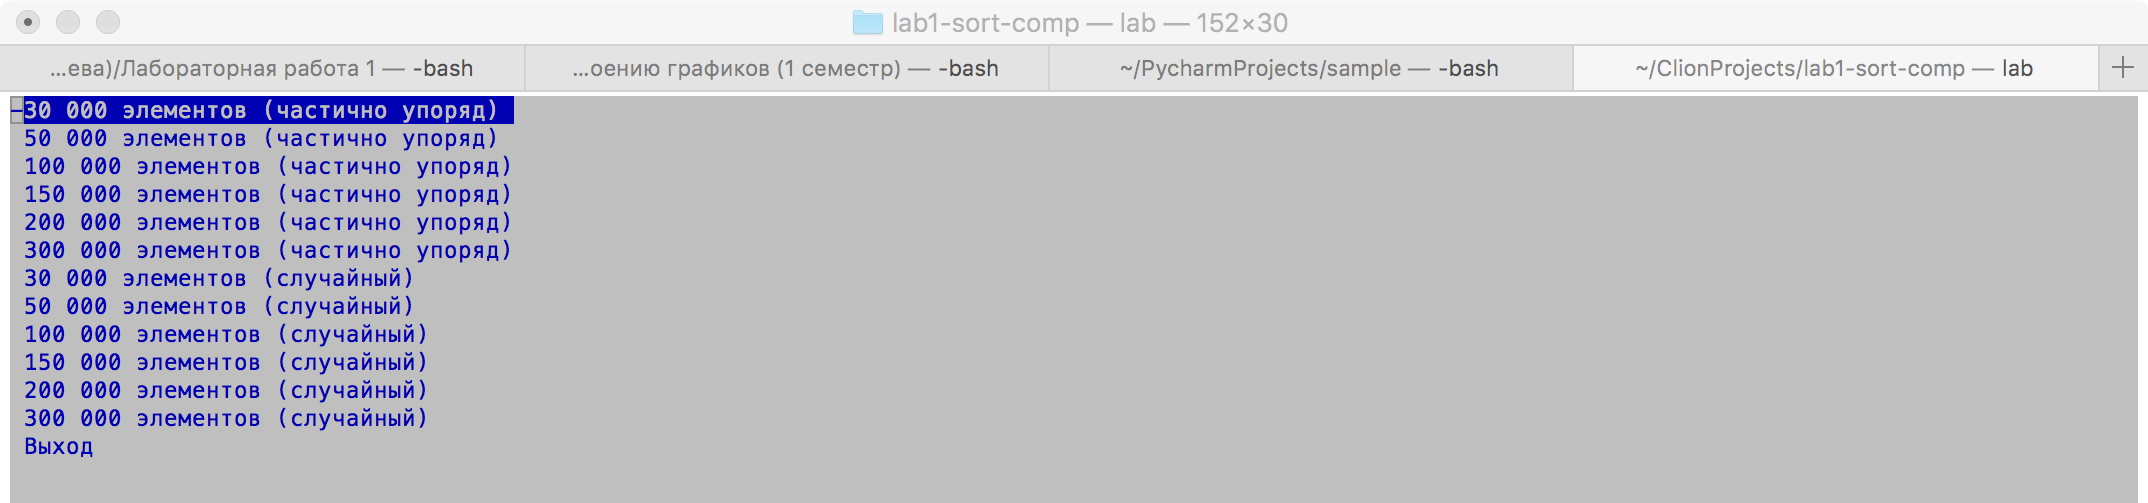
\includegraphics[width=\textwidth]{screenshot1.png}
Затем необходимо выбрать режим работы. Алгоритмы можно запускать как по одному,
так и все вместе. После окончания сортировки будет выведено время работы в секундах.\par
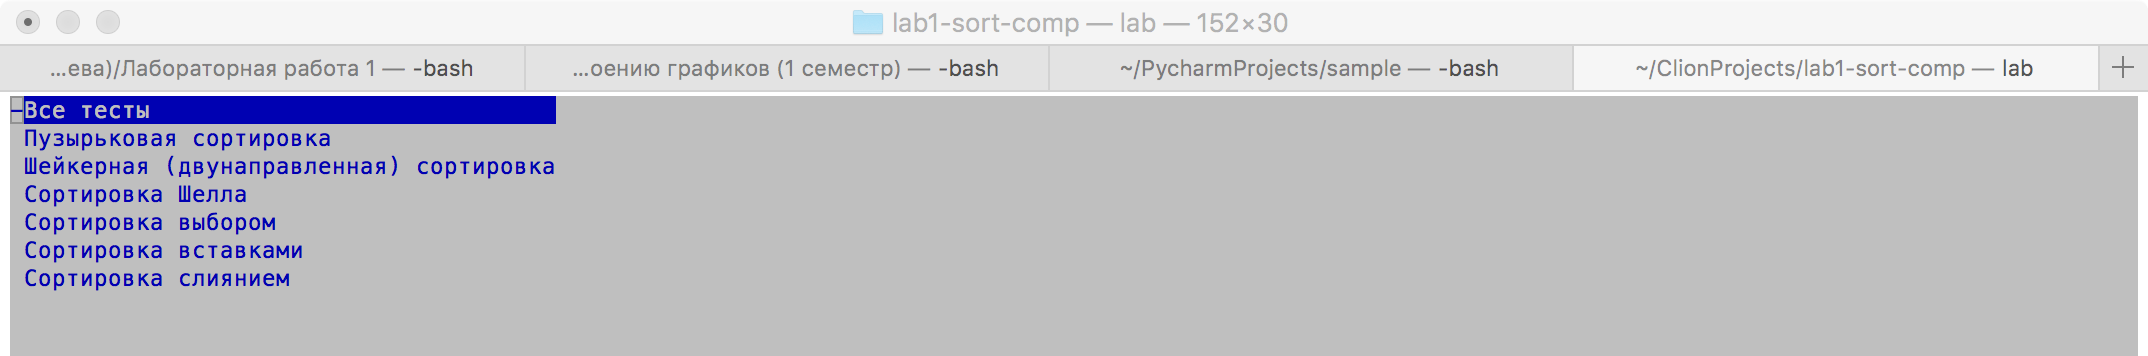
\includegraphics[width=\textwidth]{screenshot2.png}\par
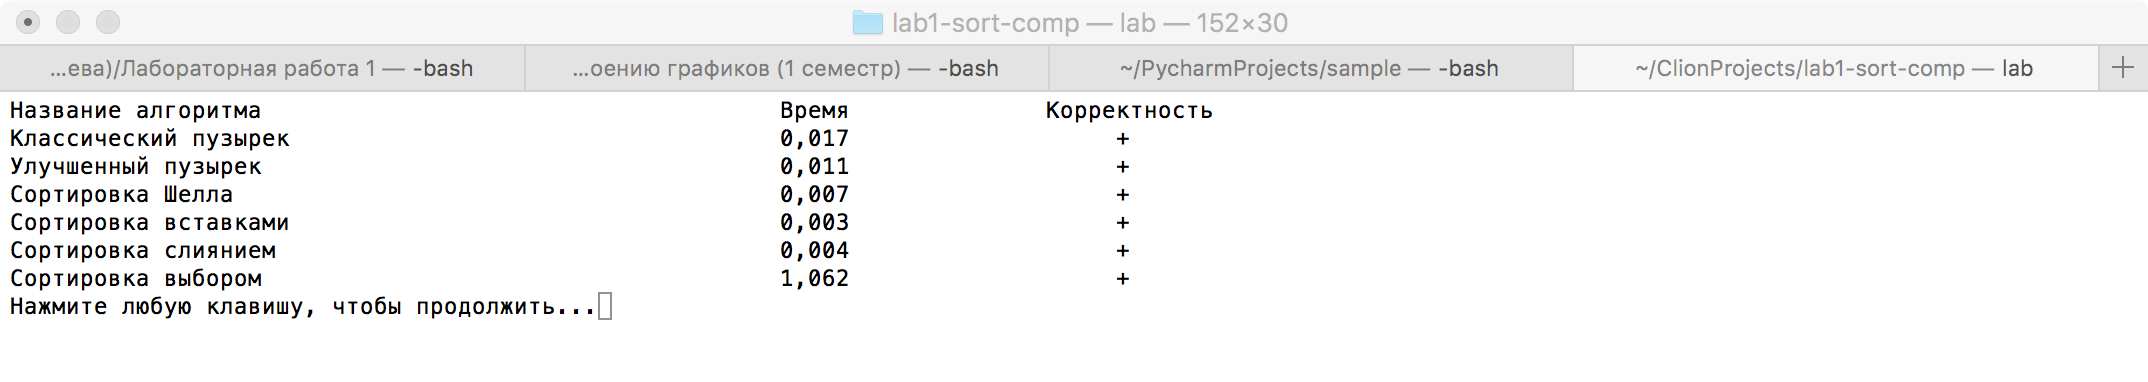
\includegraphics[width=\textwidth]{screenshot3.png}\par
\newpage
\section{Описание эксперимента}
В программе существует 2 вида наборов данных: частично упорядоченный
и абсолютно случайный. Каждый набор содержит не менее 30 000 элементов.
Тестирование на меньшем объеме данных не имеет смысла ввиду высокой
вычислительной мощности современных компьютеров. Для чистоты эксперимента
все тесты проводились на одном и том же компьютере с процессором Intel Core i5
2,6ГГц. Все остальные приложения были закрыты, чтобы не мешать работе тестового.\par
Частично упорядоченные наборы имеют следующую структуру: первые 100 элементов содержат
случайные числа от 1 до 100, следующие 100 от 101 до 200 и так далее. Случайные
наборы просто содержат случайные числа из диапазона от 0 до N.\par
Современные компьютерные системы стараются генерировать случайные числа с нормальным
распределением. За счет этого мы сможем добиться наиболее честных условий для работы
разных алгоритмов.
\newpage
\section{Обсуждение результатов}
В ходе исследования был проведен эксперимент, с помощью которого были
выявлены особенности работы алгоритмов сортировки. Результаты представлены в 
таблицах ниже.
\begin{table}[h]
\caption{Частично упорядоченные данные}
\centering
  \begin{tabular}{ | l | l | l | l | l | l | l |}
  \hline
    Алгоритм & 30k & 50k & 100k & 150k & 200k & 300k \\ \hline
    Пузырьковая сортировка & 0,017 & 0,027 & 0,054 & 0,077 & 0,099 & 0,161 \\ \hline
    Шейкерная сортировка & 0,011 & 0,018 & 0,038 & 0,055 & 0,077 & 0,122 \\ \hline
    Сортировка Шелла & 0,007 & 0,012 & 0,029 &  0,039 & 0,052 & 0,083 \\ \hline
    Сортировка вставками & 0,003 & 0,006 & 0,008 & 0,013 & 0,015 & 0,025 \\ \hline
    Сортировка слиянием & 0,004 & 0,007 & 0,014 & 0,022 & 0,029 & 0,048 \\ \hline
    Сортировка выбором & 1,064 & 2,986 & 11,876 & 26,528 & 48,269 & 107,033 \\ \hline
    \end{tabular}
\end{table}

\begin{table}[h]
\caption{Случайные данные}
\centering
  \begin{tabular}{ | l | l | l | l | l | l | l |}
  \hline
    Алгоритм & 30k & 50k & 100k & 150k & 200k & 300k \\ \hline
    Пузырьковая сортировка & 3,154 & 8,893 & 35,567 & 80,754 & 142,139 & 319,785 \\ \hline
    Шейкерная сортировка & 2,408 & 6,749 & 27,170 & 62,281 & 108,503 & 244,321 \\ \hline
    Сортировка Шелла & 2,132 & 5,085 & 23,144 & 48,592  & 94,249 & 209,012 \\ \hline
    Сортировка вставками & 0,632 & 1,740 & 6,981 & 15,498 & 27,328 & 62,970 \\ \hline
    Сортировка слиянием & 0,005 & 0,009 & 0,018 & 0,028 & 0,039 & 0,062 \\ \hline
    Сортировка выбором & 1,062 & 2,945 & 11,754 & 26,655 & 47,259 & 106,825 \\ \hline
    \end{tabular}
\end{table}

Как мы можем видеть из представленных данных, на частично упорядоченном массиве данных хорошо
показала себя сортировка вставками. Она не требует дополнительной памяти, отрабатывает за минимальное время.
Сортировка Шелла хоть и является её улучшением, показала более скромные результаты. Но этот алгоритм 
недостаточно изучен и допускает правку некоторых параметров, которые могут повлиять на его производительость.
Не самое плохое время работы продемонстрировали пузырьковые сортировки, несмотря на то, что их сложность
равна $O(N^2)$. А вот сортировка выбором - явный аутсайдер. Она требует больше всего времени.\par
Но все меняется при случайных данных. Сортировка слиянием показывает отличный результат. Сортировка выбором
так же продемонстрировала прежнее время работы. Отсюда можем сделать вывод, что структура данных мало влияет на
скорость работы этих двух сортировок. А вот другие сортировки сильно деградировали на неупорядоченном
массиве данных. В особенности пузырьковые сортировки.\par
Таким образом, в большинстве случаев стоит применять сортировку слиянием. Многие языки высокого уровня
используют её модификации в качестве алгоритмов сортировки по умолчанию. Но у скорости есть своя цена.
Сортировка слиянием требует дополнительной памяти. Если этот ресурс ограничен, стоит рассмотреть сортировку
вставками. На случайных данных она сильно уступает сортировке слиянием по времени, но гораздо более экономично
расходует память.



\newpage
% \bibliographystyle{utf8gost705u}
% \bibliography{biblio}
\printbibliography[heading=bibintoc]

\newpage
\appendix 
\section*{Приложение} 
\phantomsection
\addcontentsline{toc}{section}{{\bf Приложение}} 
\markboth{{\bf Приложение}}{{\bf Приложение}}

\begin{lstlisting}
#include <stdlib.h>
#include <time.h>
#include <stdio.h>
#include <string.h>
#include "algorithms.h"
/**
 * Классическая пузырьковая сортировка
 * @param arr Массив значений для сортировки
 * @param n Длина массива
 */
void bubble_sort(int *arr, int n)
{
    int i, l, hasChanged;
    l = n - 1;
    do
    {
        hasChanged = 0;
        for (i = 0; i < l; ++i)
        {
            if (arr[i] > arr[i + 1])
            {
                arr[i] ^= arr[i + 1];
                arr[i + 1] ^= arr[i];
                arr[i] ^= arr[i + 1];
                hasChanged = 1;
            }
        }
        l--;
    } while (hasChanged);
}
/**
 * Улучшенная сортировка пузырьком с проходом в обе стороны
 * @param arr Массив данных
 * @param n Количество элементов
 */
void better_bubble_sort(int *arr, int n)
{
    int i, start, finish, hasChanged;
    start = 0;
    finish = n - 1;
    do
    {
        hasChanged = 0;
        for (i = start; i < finish; ++i)
        {
            if (arr[i] > arr[i + 1])
            {
                arr[i] ^= arr[i + 1];
                arr[i + 1] ^= arr[i];
                arr[i] ^= arr[i + 1];
                hasChanged = 1;
            }
        }
        --finish;
        if (hasChanged)
        {
            for (i = finish - 1; i >= start; --i)
            {
                if (arr[i] > arr[i + 1])
                {
                    arr[i] ^= arr[i + 1];
                    arr[i + 1] ^= arr[i];
                    arr[i] ^= arr[i + 1];
                    hasChanged = 1;
                }
            }
            start++;
        }
    }
    while (hasChanged);
}
/**
 * Сортировка Шелла
 * @param arr Массив данных
 * @param n Количество элементов
 */
void shell_sort(int *arr, int n)
{
    int i, hasChanged;
    int d = n;
    do
    {
        d = (d + 1) / 2;
        hasChanged = 0;
        for (i = 0; i < n - d; ++i)
        {
            if (arr[i] > arr[i + d])
            {
                arr[i] ^= arr[i+d];
                arr[i + d] ^= arr[i];
                arr[i] ^= arr[i + d];
                hasChanged = 1;
            }
        }
    }
    while (d != 1 || hasChanged);
}
/**
 * Поиск минимального элемента в массиве
 * @param arr Массив
 * @param n Количество элементов
 * @return Индекс минимального
 */
int min(int *arr, int n)
{
    int i, min_idx = 0;

    for (i = 0; i < n; ++i)
    {
        if (arr[i] < arr[min_idx])
        {
            min_idx = i;
        }
    }
    return min_idx;
}
/**
 * Сортировка выбором
 * @param arr Массив данных
 * @param n Количество элементов
 */
void selection_sort(int *arr, int n)
{
    int i, j, pos;
    for (i = 0; i < n - 1; ++i)
    {
        pos = i;
        for (j = i + 1; j < n; ++j)
        {
            if (arr[pos] > arr[j])
            {
                pos = j;
            }
        }
        if (pos != i)
        {
            arr[i] ^= arr[pos];
            arr[pos] ^= arr[i];
            arr[i] ^= arr[pos];
        }
    }
}
/**
 * Сортировка вставками
 * @param arr Массив
 * @param n Количество элементов
 */
void insertion_sort(int *arr, int n)
{
    int i, j, b;
    for (i = 0; i < n - 1; ++i)
    {
        b = arr[i + 1];
        j = i;
        while ((j >= 0) && (b < arr[j]))
        {
            arr[j + 1] = arr[j];
            j--;
        }
        arr[j + 1] = b;
    }
}
/**
 * Алгоритм слияния двух упорядоченных массивов
 * @param first Первая часть
 * @param nf Размер
 * @param second Вторая часть
 * @param ns Размер
 * @param result Результат
 * @param k Количество
 */
void merge ( int * first, int nf, int * second, int ns, int * result, int k )
{
    int count = 0, i = 0, j = 0;
    first[nf] = INT_MAX;
    second[ns] = INT_MAX;
    while (count < nf + ns)
    {
        if (first[i] < second[j])
        {
            result[k + count] = first[i++];
            count++;
        } else
        {
            result[k + count] = second[j++];
            count++;
        }
    }
}
/**
 * Сортировка слиянием
 * @param arr Исходный массив
 * @param n Количество элементов
 */
void merge_sort ( int * arr, int n )
{
    int i;
    int h = 1;
    int begin;
    int nf, ns;
    int *first, *second;
    first = (int *) calloc (n, sizeof(int));
    second = (int *) calloc (n / 2 + 1, sizeof(int));
    while (h < n)
    {
        begin = 0;
        while (begin < n - 1)
        {
            nf = 0;
            for (i = 0; (i < h) && (begin + i < n); i++)
            {
                first[i] = arr[begin + i];
                nf++;
            }
            ns = 0;
            for (i = 0; (i < h) && (begin + h + i < n); i++)
            {
                second[i] = arr[begin + h + i];
                ns++;
            }
            merge(first, nf, second, ns, arr, begin);
            begin += 2 * h;
        }
        h *= 2;
    }
}
\end{lstlisting}

\end{document}
